\section{Composite marginal likelihoods}
\label{sec:piecewise}

The previous section provided a method of moments estimator
which used (i) tensor decomposition to recover conditional moments,
and (ii) matrix inversion to recover the hidden marginals.
Now we aim to improve statistical efficiency by replacing (ii) with a likelihood-based objective.

% DONE: set the stage a bit more
Of course, optimizing the original marginal likelihood is subject to local optima.
We make two observations to arrive at a convex optimization problem.
The first is that we have used tensor decomposition to recover the conditional moments,
so effectively a subset of the parameters have been fixed.
However, this alone is not enough, for the full likelihood is still non-convex.
The second insight is that we can optimize a \emph{composite likelihood objective} \cite{lindsay88composite}
rather than the full objective.

%The method of moments approach to recover parameters for each clique
  %$\sC$ presented in the previous section is easy to understand and
  %analyze, but sensitive to noise. 
%In this section we propose an alternate solution, optimizing the 
  %likelihood for each clique, that is more robust to noise.
We show that under the same conditions as \algorithmref{directed}, the
  negative composite likelihood function is strictly convex and thus
  tractable to estimate exactly.
  %guaranteeing that
  %gradient-based optimization will converge to the unique global
  %optimum.

Consider a clique $\sC = \{h_{i_1}, \cdots h_{i_m}\} \in \sG$, with
  exclusive views $\sV = \{x_{v_1}, \cdots, x_{v_m}\}$. 
The expected composite likelihood over $\Sx{\sV}$ given parameters $\mH_\sC$
with respect to the true distribution $\sM_\sV$ can be written in tensor form:
\begin{align}
  \sL_\ml %(\Sx{\sV}) 
  &= \E[\log \Pr( \Sx \sV )] \nonumber \\
  &= \E[\log \sum_{\Sh \sC} \Pr( \Sx \sV \given \Sh \sC )] \nonumber \\
  &= \E[\log \mH_\sC(\mOpp{v_1}{i_1} [x_{v_1}], \cdots, \mOpp{v_m}{i_m} [x_{v_m}])] \nonumber \\
  &= \E[\log \mH_\sC(\mOppAll[\Sx\sV])]. \label{eqn:piecewise-obj}
\end{align}
The final form is an expectation over a log of linear function of $\mH_\sC$, which is concave in
$\mH_\sC$.  But unlike maximum likelihood in fully-observed settings,
we do not have a closed form solution, so we use EM to optimize.
Since the function is convex, EM converges to a global optimum.
\algorithmref{piecewise} summarizes our algorithm.

\begin{algorithm}
  \caption{$\LearnClique$ (composite likelihood)}
  \label{algo:piecewise}
  \begin{algorithmic}
    % DONE: interface should match LearnClique from directed.tex  
    %\REQUIRE A graphical model $\sG$ satisfying \propertyref{bottleneck}, data $\sD$
    %\ENSURE Marginals $Z_\sC$ for every clique $\sC \in \sG$
    \REQUIRE Clique $\sC$ with exclusive views (\propertyref{exclusive-views}).
    \ENSURE Marginal distribution of the clique $Z_\sC$.
\STATE Identify exclusive views $x_\sV = \{x_{v_1}, \cdots, x_{v_m}\}$.
\STATE Return $\hat \mH_\sC = \arg\max_{\mH_\sC \in \Delta_{k^m-1}} \sum_{\vx \in \sD} \log \mH_\sC(\mOppAll[\Sx \sV])$.
%      Run expectation-maximization to convergence on the piecewise likelihood \eqref{eqn:piecewise}, over data $\{\vec x_\sC : x \in \sD\}$
  \end{algorithmic}
\end{algorithm}

\subsection{Statistical efficiency}

We have proposed two methods for estimating the hidden marginals $Z_\sC$ given
the conditional moments $\mOppAll$, one based on computing a simple pseudoinverse,
and the other based on composite likelihood.
Let $\hat Z^\mom_\sC$ to denote the pseudoinverse estimator and $\hat
  Z^\ml_\sC$ to denote the composite likelihood estimator.

The Cramer-Rao lower bound tells us that maximum likelihood yields the
  most statistically efficient composite estimator for $Z_\sC$ given
  access to only samples of $\Sx\sV$.\footnote{Of course, we could improve
  statistical efficiency by maximizing the likelihood of all of $\vx$, but
  that would again lead to a non-convex optimization problem.}
But can we quantify the \emph{relative efficiency} of the pseudoinverse
  estimator compared to the composite likelihood estimator?
We turn to asymptotic statistics to answer this question. 

To begin, let us compute the asymptotic variances of the two estimators. 
Note that $\hat Z_\sC$ is constrained to lie on the simplex
  $\Delta_{k^m-1}$ and that $M_\sV$ is similarly constrained to lie on
  the simplex $\Delta_{d^m-1}$. 
To handle these constraints, we reparameterize our problem in
  terms of $\tZ_\sC \in [0,1]^{k^m-1}$ and $\tM_\sV \in [0,1]^{d^m-1}$.
  The first $k^m -1$ terms of $\tZ_\sC$ and $Z_\sC$ are equal, and the
  last element, $Z_\sC[k, \ldots, k]$ picks up the slack to make $Z_\sC$
  sum to 1:
\begin{align*}
  Z_\sC[\vi] &= \left\{
    \begin{array}{ll}
      1 - \sum_{\vi' \prec \vk} \tilde Z_\sC[\vi'] & \vi = \vk \\
      \tilde Z_\sC[\vi] & \text{otherwise.}
      \end{array}
      \right.,
\end{align*} 
where $\vk = (k, \ldots, k)$ is the $m$-dimensional vector of all $k$s. 
$M_\sV$ is similarly defined in terms of $\tM_\sV$.

Now, abusing notation slightly by using the vectorized forms of $M_\sV
\in \Re^{d^m}$, $\tM_\sV \in \Re^{d^m-1}$, $Z_\sC \in \Re^{k^m}$, $\tilde Z_\sC \in \Re^{k^m-1}$
and the matrix form of $\mOppAll \in \Re^{d^m \times k^m}$, the marginal
distribution can be expressed as follows,
\begin{align*}
  \tM_\sV 
        &= \mOppAll_{\neg d} Z_\sC \\
        &= \mOppAll_{\neg \bd, \neg \vk} \tilde Z_\sC + \mOppAll_{\neg \bd, \vk} (1 - \ones^\top \tilde Z_\sC) \\
        &= \underbrace{(\mOppAll_{\neg \bd, \neg \vk} -  \mOppAll_{\neg \bd, \vk}\ones^\top)}_{\mOppTAll} \tilde Z_\sC + \mOppAll_{\neg \bd, \vk}.
        % &= \mOppTAll \tilde Z_\sC + \mOppAll_{\vk},
\end{align*}
where $\mOppAll_{\neg \bd, \neg \vk} \in \Re^{d^m -1 \times k^m - 1}$ matrix containing the
first $d^m-1$ rows and first $k^m-1$ columns of $\mOppAll$, $\mOppAll_{\neg \bd, \vk} \in \Re^{d^m}$ is the last column. 

We are now ready to study the asymptotic properties of $Z_\sC$ through
$\tZ_\sC$ and $\tM_\sV$.

\providecommand{\hatt}[1] {\hat{\tilde{#1}}}
\begin{lemma}[Asymptotic variances]
  \label{lem:mom-pw-variance}
  The asymptotic variance of $\hatt Z^\mom_{\sC}$ based on composite likelihood and 
  $\hatt Z^\ml_{\sC}$ based on composite likelihood are respectively,
  \begin{align*}
    \Sigma^{\mom} &= \mOppTAlli \tilde\Sigma_\sV \mOppTAllit \\
    \Sigma^{\ml} &= \Sigmamom - \frac{\Sigmamom (\mOppTAllt \ones)(\mOppTAllt \ones)^\top \Sigmamom}{\frac{1 - \ones^\top \tM_\sV}{\ones^\top \tM_\sV} + (\mOppTAllt \ones)^\top \Sigmamom (\mOppTAllt \ones)},
  \end{align*}
  where $\tilde \Sigma_\sV = \tD_\sV (I - \tD_\sV)$, the variance of $\tM_\sV$ and $\tD_\sV = \diag(\tM_\sV)$.
\end{lemma}
\begin{proof}
  The above two results follow by direct application of the delta-method
  \cite{vaart98asymptotic}. Refer to \appendixref{pw-proof} for
  a complete derivation.
\end{proof}

%%%%%%%%%%%%%%%%%%%%%%%%%%%%%%

The following corollary (proved in \appendixref{pw-proof}) shows that
the gap between the two estimators closes at a rate of $k^m$.
\begin{corollary}[Asymptotic efficiency]
  \label{cor:efficiency}
The pseudoinverse estimator is strictly less efficient
than the composite likelihood estimator in that 
\begin{align*}
e^\mom &\eqdef 
    \frac{1}{k^m-1} \Tr(\Sigmaml\Sigmamomi ) \\
        &= 1 - \frac{1}{\bar k} \frac{ \ones_{\bar k}^\top \widetilde\Sigma_\sV \ones_{\bar k}}{\frac{1 - \ones^\top \tM_\sV}{\ones^\top \tM_\sV} + \ones_{\bar k}^\top \widetilde\Sigma_\sV \ones_{\bar k}} \\
    &< 1.
\end{align*}

When $M_\sV$ is close to the uniform distribution, i.e. $M_\sV \approxeq \frac{1}{d^m} \ones \implies \tilde\Sigma_\sV = \frac{d-1}{d^2} I$, we get that 
\begin{align*}
e^\mom 
    &= 1 - \frac{(d^m -1)^2}{ (d^m)^2 + (k^m-1)(d^m -1)^2} 
    &\simeq 1 - \frac{1}{k^m}.
\end{align*}
\end{corollary}

\figureref{cl-hmm} compares the parameter recovery error of the
  pseudoinverse estimator and the composite likelihood estimator.
Empirically, we observe that using the composite likelihood estimator
indeed leads to more accurate estimates.

% Visualize
% To visualize this phenomenon, note that the pseudoinverse estimator can be written
% as $\hat Z_\sC = \argmin_{Z_\sC} \|Z_\sC \mOppAll - M_\sV \|_F^2$.
% \figureref{piecewise-objective} plots the compares the objective values for
% different choices of the $\pi$ parameter in a hidden Markov model
% (\figureref{examples-hmm}) with 2 states ($k=2$) and $d=10$ dimensions.
% Note that the negative log-likelihood objective is more
% strongly convex than the pseudoinverse objective.
% \todo{this is perhaps misleading, you could get the plot with the same with $100000000000 x^2$ and $x^2$.
% Let's talk about this.  If can't fix, remove.
% }

\begin{figure}
  \centering
  %  \subfigure[Comparing the piecewise objective with the moment-matching objective] {
  %    \label{fig:piecewise-objective}
  %    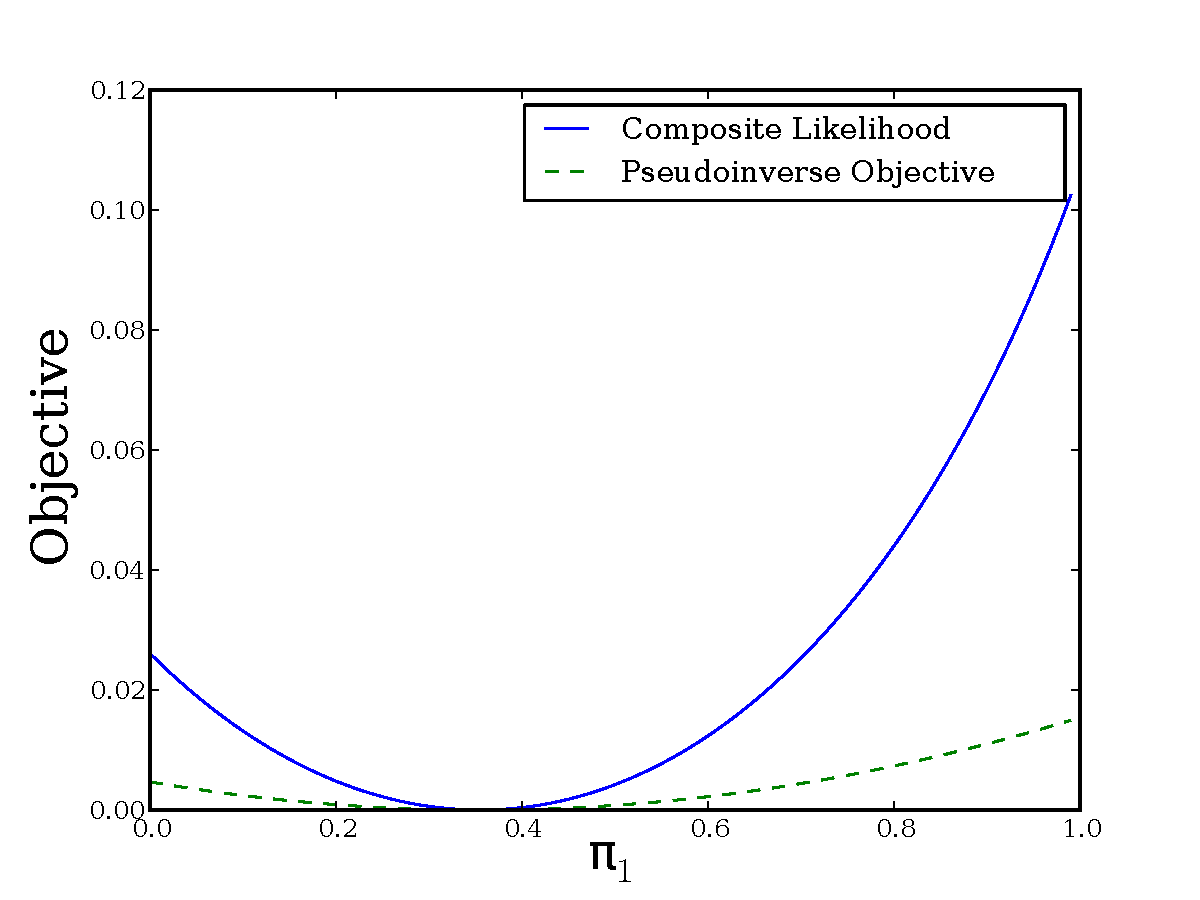
\includegraphics[width=0.45\columnwidth]{figures/piecewise-objective.pdf}
  %  }
%  \subfigure[Directed grid model] {
%    \label{fig:examples-grid}
%    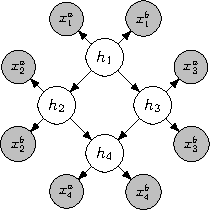
\includegraphics{figures/grid.pdf}
%  }
%  \subfigure[] {
  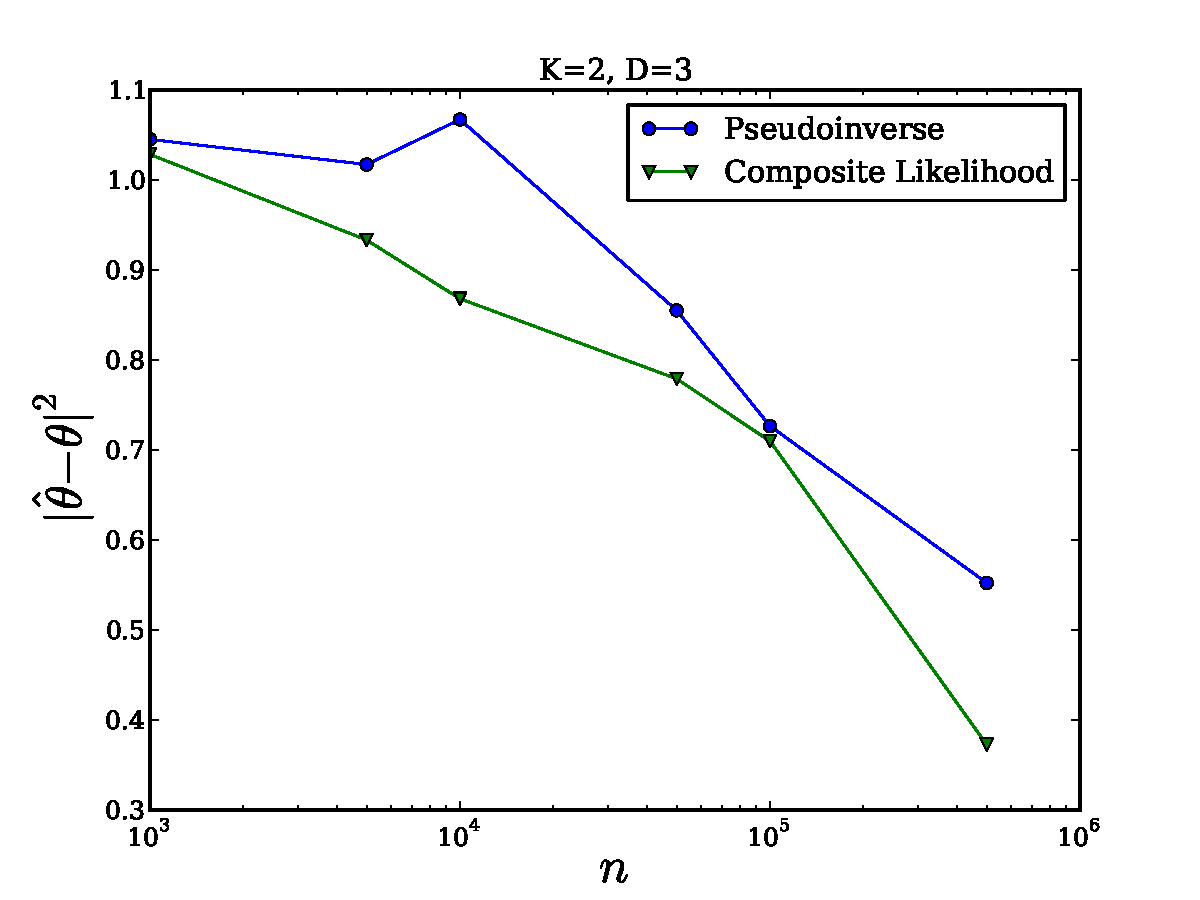
\includegraphics[width=0.8\columnwidth]{figures/hmm-2-3.pdf}
%  }
  \caption{Parameter estimation error when recovering parameters for a Hidden
  Markov Model with $k=2$ states and $d=3$ emissions using two types of estimators.}
    \label{fig:cl-hmm}
\end{figure}
